% Chapter 3

\chapter{Các nguồn chia sẻ dữ liệu} % Main chapter title

\label{Chapter3}

\section{HERE Real-time Traffic}
HERE Real-time Traffic là một dịch vụ của HERE Technologies - một công ty nổi tiếng và có kinh nghiệm trong việc cung cấp các dịch vụ về bản đồ và vị trí. Dịch vụ trên giúp người dùng có thể xác định vị trí, thời gian và lý do tắc nghẽn giao thông xảy ra bằng cách cung cấp tình trạng giao thông và các sự cố từng phút. Nguồn dữ liệu của dịch vụ được cung cấp và phân tích từ nhiều nguồn tổng hợp như cảm biến của ôtô, các cảm biến cố định trên đường hoặc từ các thiết bị sử dụng các ứng dụng của công ty. Năm 2017, HERE thông báo dịch vụ HERE Real-time Traffic cũng đã hỗ trợ ở Việt Nam.\cite{HERE}

\begin{figure}[!ht]
	\begin{center}
		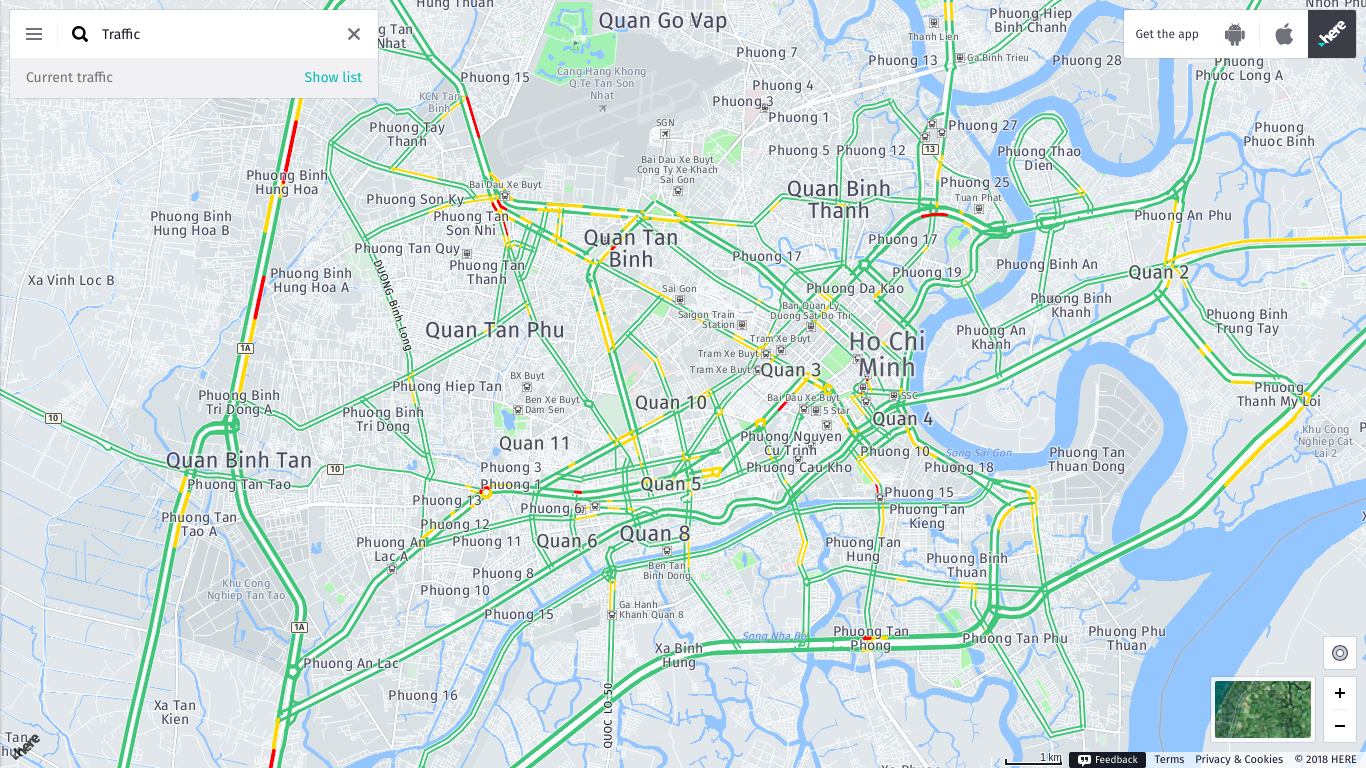
\includegraphics[width=1.0\textwidth]{images/here_maps.png}
	\end{center}
	\caption{HERE Real-time Traffic được sử dụng trên Here maps}
\end{figure}

Mặc dù được HERE giới thiệu rằng dịch vụ cung cấp nguồn dữ liệu thời gian thực và có độ chính xác cao. Tuy nhiên khi tiến hành tìm hiểu và nghiên cứu dịch vụ bằng cách sử dụng các API để lấy dữ liệu giao thông và so sánh với tình trạng giao thông ở một số thời điểm thực tế, nhóm nhận thấy dữ liệu dịch vụ cung cấp vẫn chưa thật sự có độ chính xác cao ở Việt Nam, cụ thể là thành phố Hồ Chí Minh. Vì thế, nhóm quyết định tạm dừng việc sử dụng HERE Real-time traffic lấy dữ liệu giao thông và tìm hiểu một số nguồn cung cấp dữ liệu khác.
\section{Smart BK Traffic}
Hệ thống giao thông thông minh (Smart BK Traffic) là hệ thống được nhóm Intelligent Transportation Systems Group (ITSG) tại trường Đại học Bách Khoa phát triển. Hệ thống được xây dựng để thu thập xử lý tín hiệu GPS từ xe hơi, xe taxi, xe buýt, thiết bị di động; đồng thời cung cấp dữ liệu đã được xử lý đến các ứng ụng web và điện thoại thông minh theo thời gian thực.

\begin{figure}[!ht]
	\begin{center}
		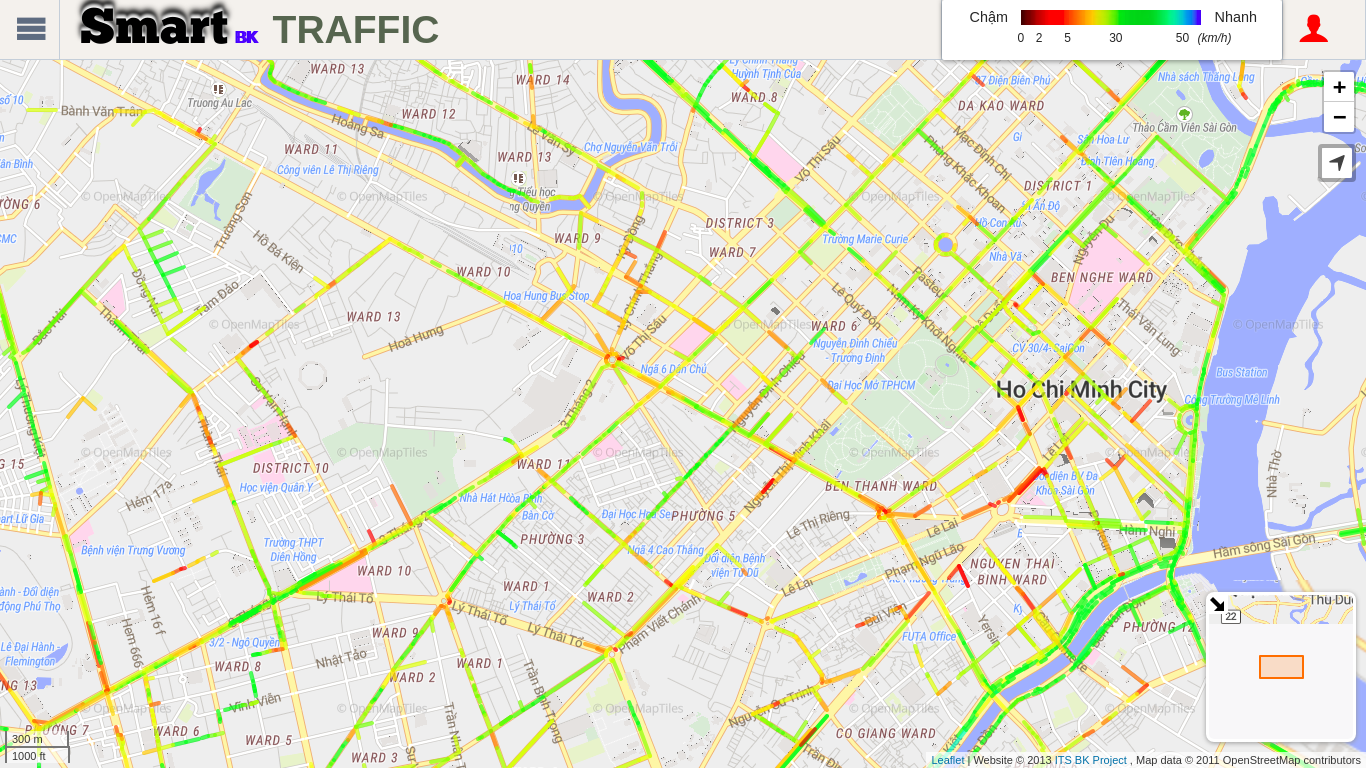
\includegraphics[width=1.0\textwidth]{images/smartbktraffic.png}
	\end{center}
	\caption{Website của hệ thống Smart BK Traffic - 17:45 08/12/2018}
\end{figure}

Sau một thời gian tìm hiểu và đánh giá, nhóm nhận thấy dữ liệu do hệ thống Smart BK Traffic cung cấp tương đối chính xác đối với tình trạng giao thông của thành phố Hồ Chí Minh. Mặc dù dữ liệu vẫn bị thiếu ở một số tuyến đường nhưng nhìn chung vẫn khá đầy đủ. Do đó, nhóm quyết định sử dụng nguồn dữ liệu này, kết hợp với nguồn dữ liệu crowdsourcing để có thể khai phá, đưa ra dự đoán tình hình giao thông ở những đoạn đường bị thiếu nhằm bổ sung vào những thiếu sót mà hệ thống đang có. Chi tiết về cách thu thập cũng như sử dụng dữ liệu sẽ được nhóm trình bày vào chương 4.
\section{Dữ liệu từ cộng đồng (Crowdsourcing)}
Như đã trình bày ở trên, nguồn dữ liệu thu thập được từ cộng đồng là một nguồn dữ liệu quan trọng và không thể thiếu trong quá trình làm đề tài. Một ví dụ cho tính hiệu quả của việc sử dụng nguồn dữ liệu cộng đồng ở Việt Nam là hệ thống VOV Giao thông 91Mhz của Đài tiếng nói Việt Nam, với cách thức thông báo tình trạng giao thông thông qua sóng radio với nguồn thông tin chính xác đến từ các tài xế lái xe, từ đó giúp cho các tài xế khác có thể điều chỉnh lộ trình của mình cho phù hợp, tránh đi những tuyến đường bị kẹt xe. Tuy nhiên việc sử dụng dữ liệu cộng đồng như thế vẫn còn rất nhiều hạn chế, cho nên cần một giải pháp khác để khai thác, sử dụng hiệu quả nguồn dữ liệu từ cộng đồng hơn. Một vài nhóm nghiên cứu nước ngoài cũng đã thực hiện một số công trình nghiên cứu về việc áp dụng kỹ thuật thu thập dữ liệu cộng đồng (crowdsourcing) để giải quyết các bài toán thu thập dữ liệu nói chung, và giao thông nói riêng \cite{CROWND1} \cite{CROWND2} \cite{CROWND3} \cite{CROWND4}. Từ những nghiên cứu nói trên, nhóm kết hợp với hai nhóm khác cũng làm đề tài liên quan đến giao thông để xây dựng hệ thống cung cấp thông tin giao thông theo thời gian thực cho người dùng thông qua ứng dụng di động, với nguồn dữ liệu đến từ chính cộng đồng người dùng của ứng dụng.